% \documentclass{acm_proc_article-sp}
\documentclass{sig-alternate-2013}
\usepackage{url}


\begin{document}

\title{Kimbee: A Speech Therapy Application For Children}

\numberofauthors{1}
\author{
    \alignauthor
    \vspace*{-0.3in}
        Ryan Drapeau \hspace{3.0cm}
        Nick Huynh \hspace{3.0cm}
        Aaron Nech \\
    \affaddr{
        \hspace{0.3cm}
        University of Washington \hspace{1.4cm}
        University of Washington \hspace{1.4cm}
        University of Washington \hspace{0cm}
        } \\[7 pt]
    \email{{\centering \{drapeau, huynick, necha\}@cs.washington.edu}}
}

\maketitle

\begin{abstract}

We have developed an application named {\em Kimbee} that aims to help the process of speech therapy in young children. Speech therapies are often expensive for schools and parents to maintain, especially with younger children who require more time than others. Our application does not replace the speech therapist, rather it supplements the therapy. Instead of being limited to short sessions, therapists can use {\em Kimbee} to have their students work at home as well as in the classroom. The therapist can then monitor the child's progress through our application and use this newly gained information to further tailor the therapy to individual students. This will save both time and money for school districts and parents who are paying for their child's therapy.

\end{abstract}

\section{Introduction}

The purpose of this paper and project is to make speech therapy more effective in English speaking children from age 5 to age 12. Children in this age group tend to average over a year involved in weekly speech therapy meetings to overcome a speech disorder \cite{Kreider:Intro}. It is also common for therapists to spend most of their time with students during these sessions or in the classroom because it is often hard to work with children remotely. A session usually consists of having the child repeat words back to the therapist in order to target a specific sound or phoneme. Common speech impediments in children are often caused by functional speech disorders, or trouble learning to make specific speech sounds \cite{Brown:Children}.

We chose to focus on `R' sounds as they are one of the more common mispronunciations found in our target age group \cite{Dodd:Children}. Most `R' disorders will commonly pronounce words as if the `R' was a `W'. An example would be pronouncing the word {\em ``rabbit''} as {\em ``wabbit''}. We use similar techniques as therapists use in their sessions in our online application. By having the child or user repeat a target several times until he or she is able to pronounce it correctly, we are emulating the in person setting that they are used to. Each time a word is spoken, an audio recording of the speech is documented and saved for the therapist to analyze at a later time. This process is then wrapped in game setting to make the process of saying and repeating words more enjoyable for children. This helps supplement the therapy, rather than aiming to replace it. We hope that this will cause a decrease in the amount of time that children will need to spend in therapy, which will help save the school district or parents more money.

We will also show how our application is general enough that it can be expanded to beyond `R' sounds making it applicable to any of the 36 different types of speech impediments. This will make our application a useful tool to use in all therapies that are being used with children's speech.

\section{Related Work}

With the widespread use of the tablet and increasing availability of the Internet, several applications have been developed that are similar to {\em Kimbee}. Researchers at the University of Zaragoza have created a standalone tablet application that aims to remove the therapist from the treatment \cite{Carlos:Vocaliza}. The researchers created an application for children to speak words and receive feedback on whether the word they said matches what was on the screen. The model they used also requires the student to train his or her voice in order for it to be recognized and processed correctly. Because of this, the amount of time it would take a new student to get started is significant. Their application currently only supports the Spanish language, which would not be of much help to English speaking students. Our project's scope is almost much narrower. Our focus is to help the therapist spend higher quality time with his or her students by giving them additional information from the student's work outside the sessions.

There has also been work designing an elaborate collaboration between students and therapists. The European Department for Speech, Music, and Hearing published an article describing a new system and plan for speech therapy in children \cite{Oster:EU}. This paper addresses the fact that having a visual feedback system is essential for children to be able to learn and improve their speech. However, this paper fails to provide an implementation or describe one further than a few diagrams. The real-time feedback system and long-term statistics described are very similar to what we have implemented in {\em Kimbee}.

In addition to the work previously listed, there has also been a lot of development for speech therapy applications on Apple's iTunes Store and Android's Google Play Store \cite{Mobile:Apps}. A quick search for speech therapy mobile applications will reveal many results. However, most of these applications fail to incorporate a therapist into the learning model, which we believe is essential for helping the child overcome his or her disorder.

\section{Implementation}

We will now introduce our implementation and solution to the problem posed for children's speech therapy. Before we started designing {\em Kimbee}, we met with speech pathologist Richard Kreider to discuss what features would be needed for a system like this to work \cite{Kreider:Intro}. Mr. Kreider has over 25 years of experience working with children to overcome their speech disorders. Mr. Kreider talked about how this application would need to have a way for children to practice at home as additional work as well as a way for him to track the progress of his students over time. As these were the two most important features Mr. Kreider discussed, we designed Kimbee around them as core features.

\begin{figure}[t!]
  \centering
  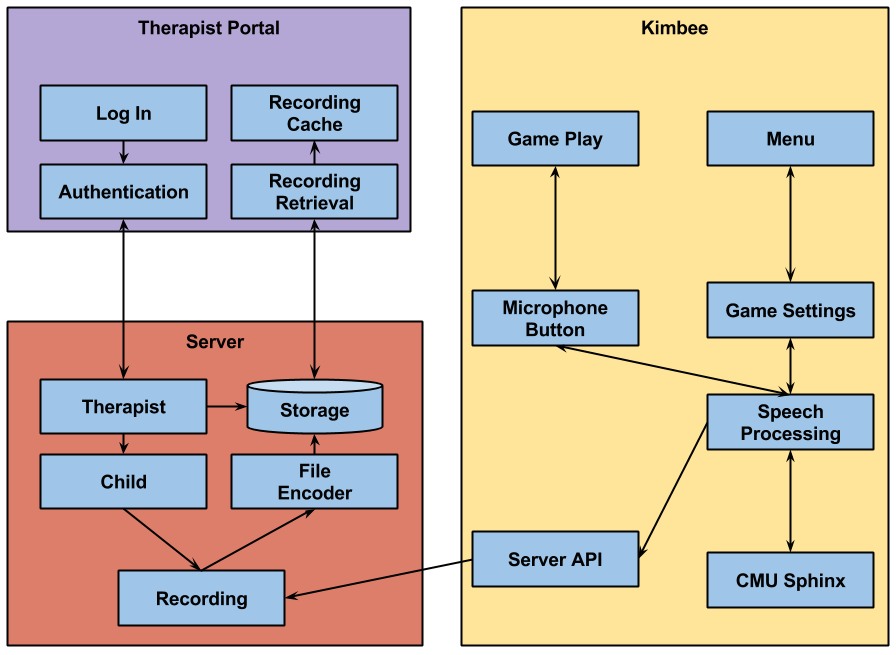
\includegraphics[keepaspectratio, width=0.48\textwidth]{tech_figure.png}
  \caption{Tech Figure}
  \label{fig:tech}
\end{figure}

\subsection{User Flow}

\subsection{Game ({\secit Kimbee})}

\subsection{Therapist Portal}

\section{Results}

\section{Conclusion}

\section{Future Work}

There are a few ways that we can expand on {\em Kimbee}. We plan on deploying the project for use in the Arlington Public School District to see how children respond and learn from {\em Kimbee} along with how experienced speech therapists use {\em Kimbee} to aid the therapy process. Along with this, we can also expand on the application itself by targeting speech sounds past the `R' and `W' sound replacement. We can also enhance the child's experience by adding more mini games for the child to play and a token system for children to spend the honey they collect on aesthetics for the bee character.

\section{Acknowledgments}

We would like to thank Richard Kreider of the Arlington Public School District for meeting with us to discuss the viability and details of our project when it was in its developing stages and then again to discuss improvements when Kimbee was almost finished \cite{Kreider:Intro,Kreider:Results}.

\bibliographystyle{abbrv}
\bibliography{sigproc}

\balancecolumns

\end{document}
